\documentclass{article}

\usepackage{fancyhdr}
\usepackage{extramarks}
\usepackage{amsmath}
\usepackage{amsthm}
\usepackage{amsfonts}
\usepackage{tikz}
\usepackage[plain]{algorithm}
\usepackage{algpseudocode}
\usepackage{graphicx}
\usepackage{float}

\usetikzlibrary{automata,positioning}

%
% Basic Document Settings
%

\topmargin=-0.45in
\evensidemargin=0in
\oddsidemargin=0in
\textwidth=6.5in
\textheight=9.0in
\headsep=0.25in

\linespread{1.1}

\pagestyle{fancy}
\lhead{\hmwkAuthorName}
\chead{\hmwkClass\: \hmwkTitle}
\rhead{\firstxmark}
\lfoot{\lastxmark}
\cfoot{\thepage}

\renewcommand\headrulewidth{0.4pt}
\renewcommand\footrulewidth{0.4pt}

\setlength\parindent{0pt}

%
% Create Problem Sections
%

\newcommand{\enterProblemHeader}[1]{
    \nobreak\extramarks{}{Question \arabic{#1} continued on next page\ldots}\nobreak{}
    \nobreak\extramarks{Question \arabic{#1} (continued)}{Question \arabic{#1} continued on next page\ldots}\nobreak{}
}

\newcommand{\exitProblemHeader}[1]{
    \nobreak\extramarks{Question \arabic{#1} (continued)}{Question \arabic{#1} continued on next page\ldots}\nobreak{}
    \stepcounter{#1}
    \nobreak\extramarks{Question \arabic{#1}}{}\nobreak{}
}

\setcounter{secnumdepth}{0}
\newcounter{partCounter}
\newcounter{homeworkProblemCounter}
\setcounter{homeworkProblemCounter}{1}
\nobreak\extramarks{Question \arabic{homeworkProblemCounter}}{}\nobreak{}

%
% Homework Problem Environment
%
% This environment takes an optional argument. When given, it will adjust the
% problem counter. This is useful for when the problems given for your
% assignment aren't sequential. See the last 3 problems of this template for an
% example.
%
\newenvironment{homeworkProblem}[1][-1]{
    \ifnum#1>0
        \setcounter{homeworkProblemCounter}{#1}
    \fi
    \section{Question \arabic{homeworkProblemCounter}}
    \setcounter{partCounter}{1}
    \enterProblemHeader{homeworkProblemCounter}
}{
    \exitProblemHeader{homeworkProblemCounter}
}

%
% Homework Details
%   - Title
%   - Due date
%   - Class
%   - Section/Time
%   - Instructor
%   - Author
%

\newcommand{\hmwkTitle}{Deep Learning for Natural Language Processing}
\newcommand{\hmwkDueDate}{January 11, 2019}
\newcommand{\hmwkClass}{Deep Learning}
\newcommand{\hmwkClassTime}{}
\newcommand{\hmwkClassInstructor}{}
\newcommand{\hmwkAuthorName}{\textbf{Acher Clément}}

%
% Title Page
%

\title{
    \vspace{2in}
    \textmd{\textbf{\hmwkClass:\ \hmwkTitle}}\\
    \normalsize\vspace{0.1in}\small{Due\ on\ \hmwkDueDate}\\
    \vspace{0.1in}\large{\textit{\hmwkClassInstructor\ \hmwkClassTime}}
    \vspace{3in}
}

\author{\hmwkAuthorName}
\date{}

\renewcommand{\part}[1]{\textbf{\large Part \Alph{partCounter}}\stepcounter{partCounter}\\}

%
% Various Helper Commands
%

% Useful for algorithms
\newcommand{\alg}[1]{\textsc{\bfseries \footnotesize #1}}

% For derivatives
\newcommand{\deriv}[1]{\frac{\mathrm{d}}{\mathrm{d}x} (#1)}

% For partial derivatives
\newcommand{\pderiv}[2]{\frac{\partial}{\partial #1} (#2)}

% Integral dx
\newcommand{\dx}{\mathrm{d}x}

\newcommand\inner[2]{\langle #1, #2 \rangle}
\DeclareMathOperator{\Tr}{Tr}


% Alias for the Solution section header
\newcommand{\solution}{\textbf{\large Solution}}

% Probability commands: Expectation, Variance, Covariance, Bias
\newcommand{\E}{\mathrm{E}}
\newcommand{\Var}{\mathrm{Var}}
\newcommand{\Cov}{\mathrm{Cov}}
\newcommand{\Bias}{\mathrm{Bias}}

\begin{document}

\maketitle

\pagebreak

\begin{homeworkProblem}
  Let's show that

  $$
 W ^ { \star } = \underset { W \in O _ { d } ( \mathbb { R } ) } { \operatorname { argmin } } \| W X - Y \| _ { F } = U V ^ { T } , \text { with } U \Sigma V ^ { T } = \operatorname { SVD } \left( Y X ^ { T } \right)
  $$

  
 Let $W \in O _ { d } ( \mathbb { R }$. We first notice that :
  \begin{align*}
    \| W X - Y \|^2_{F} &= \| WX \|^2_F + \| Y \|^2_F - 2 \inner{WX}{Y}\\
    &= \| X \|^2_F + \| Y \|^2_F - 2 \inner{WX}{Y} && (W \in O _ { d } ( \mathbb { R } ))
  \end{align*}

  Where $\inner{WX}{Y} = \Tr{((WX)^TY)} = \Tr{(W^T Y X^T)}$. Hence,
  \begin{align*}
    \underset { W \in O _ { d } ( \mathbb { R } ) } { \operatorname { argmin } } \| W X - Y \| _ { F } &= \underset { W \in O _ { d } ( \mathbb { R } ) } { \operatorname { argmin } } \| W X - Y \|^2 _ { F }\\
    &= \underset { W \in O _ { d } ( \mathbb { R } ) } { \operatorname { argmax } } \Tr{(W^T Y X^T)}
  \end{align*}
  Let $U \Sigma V ^ { T }$ the SVD decomposition of $Y X^T$.
  \begin{align*}
    \Tr{(W^T Y X^T)} &= \Tr{(W^T U \Sigma V^T)}\\
    &= \Tr{(V^T W^T U \Sigma)}
  \end{align*}

  Let $Z = W^T U \Sigma$. $Z$ is orthogonal as the product of orthogonal
  matrices. $\Tr{(Z \Sigma)} = \sum _ { i = 1 } ^ { n } Z _ { i , i } \Sigma _ {
    i , i }$. $(\Sigma_{i, i})_i$ are non-negative and $Z$ is orthogonal hence the
  previous quantity is maximized if $Z_{i, i} = 1$ which means that $Z = I_n$.
  We then conclude that $W^* = U V^T$.
  
\end{homeworkProblem}

\begin{homeworkProblem}
 We test the sentence classification task using bot the average of word vectors
 and the weighted-average based on the idf.

 We get the following results :

\begin{center}
\begin{tabular}{|c|c c|}
  \hline
  Dataset & Average & IDF \\
  \hline
  Train & 0.4992 & 0.4993 \\
  Dev & 0.4405 & 0.4233 \\
  \hline
\end{tabular} 
\end{center}

We get slightly better results using the average of word vectors.\\

A classifier based on SVM was also trained and achieves similar results. Random
forest was also tested, but even after tweaking the hyperparameters, it was
still overfitting the train dataset.

\end{homeworkProblem}

\begin{homeworkProblem}
  We use the categorical cross-entropy loss function :
  $$ 
- \sum_{o=1}^{N}\sum _ { c = 1 } ^ { 5 } y _ { o , c } \log ( p _ { o , c } )
  $$
  Where :
  \begin{itemize}
  \item $N$ is the number of observations
  \item $y$ is the true distribution : $y_{o, c} = 1$ if observation $o$ is of
    class $c$.
  \item $p$ is the predicted distribution - i.e. the output of the model. $p_{o,
    c}$ is the probability of observation $o$ to be from class $c$ according to
  the model.
  \end{itemize}
\end{homeworkProblem}

\begin{homeworkProblem}
 
  We train a classifier based on a the LSTM model. Without using pretrained
  embedding vectors, the model is quite far from beating the logistic
  regression. Also note that it overfits very quickly : to avoid this the model
  was just trained on 2 epochs. See Figure \ref{lstm}. After 2 epochs, the dev loss starts to increase.
  
\begin{figure}[H]
  \begin{center}
    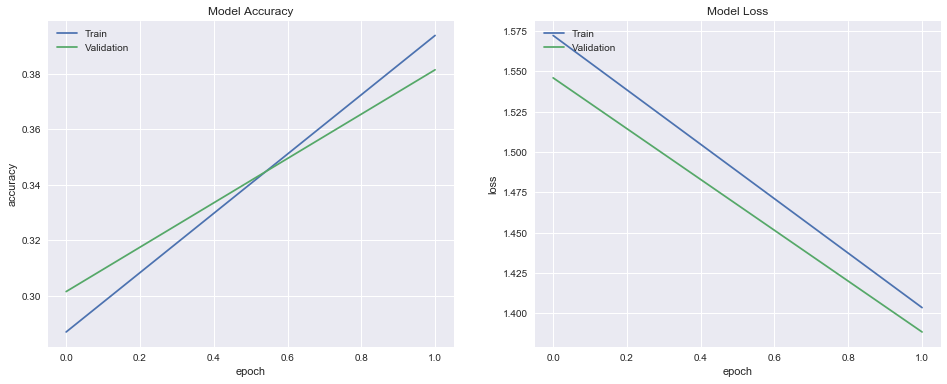
\includegraphics[width=0.9\linewidth]{./img/lstm.png}
    \caption{\label{lstm} Loss and accuracy for the LSTM model}
  \end{center}
\end{figure}

\end{homeworkProblem}

\begin{homeworkProblem}
  Given the poor results that we get from simply using a LSTM, we decide to use
  the pretrained Fasttext vectors as embeddings.
  We still use LSTM cells, but we put a 1D convolutionnal layer before, which
  gives a convolutionnal LSTM network. Another nice advantage of this solution
  is that with the pretrained embeddings and the maxpool layer, training is much
  faster.\\

  See Figure \ref{cnn_lstm} for the accuracy and loss plots. This models also
  tends to overfit : we stop the training after 6 epochs. This models gets
  better results than the vanilla LSTM model, but does not perform better than
  the logistic regression on the validation dataset.

  \begin{figure}
  \begin{center}
    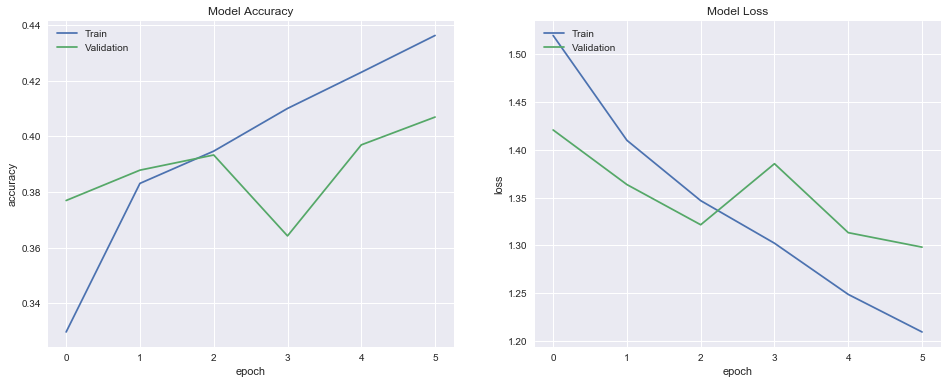
\includegraphics[width=0.9\linewidth]{./img/lstm_fast.png}
    \caption{\label{cnn_lstm} Loss and accuracy for the CNN-LSTM model}
  \end{center}
\end{figure}

\end{homeworkProblem}

\end{document}